\section{Reinforcement Learning}

Reinforcement Learning refers to a kind of Machine Learning method in which an agent learns to solve a given task by maximizing the received reward signal. Where the agent represents the reinforcement learning algorithm.\\

%The environment refers to the object the agent is acting on, while the agent represents the reinforcement learning algorithm.

%Learns to solve tasks by maximizing the reward signal it gets

\begin{figure}[H]
  \centering
  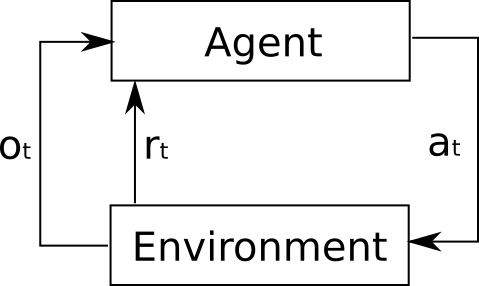
\includegraphics[width=300px]{Images/rl_agent.png} 
  \caption{Agent: reinforcement learning algorithm; Environment: object the agent is acting on; $a_t$ action the agent performce in the environment; $o_t$: observation (current state) of the envirionment the agent receives; $r_t$ reward signal the agent receives from the environment}
  \label{fig:reinforcement_learning}
\end{figure}



The Figure \ref{fig:reinforcement_learning} shows the interaction of the agent with the environment where the environment refers to the object the agent is acting on. As initial state the agent receives the observation $o_t$ of the environment at time $t = 0$. The observation $o_t$ can be the complete state of the environment or just a subset of it.
%(For example when learning the movement of a roberter the observation could be the view from the robot onto the environment.)
The agent then, based on the obervation $o_t$, performce an action $a_t$ in the environment, choosen from a set of possible actions (e.g. moving to the right or moving to the left). After performing the action $a_t$ the agent receives the new observation $o_{t+1}$ of the environment and also the reward signal $r_{t+1}$ which evaluates how good the choosen action was.
Based on the two new information the agent again choose an action $a_t$. The loop continuouse until the environment sent a termination state.\\

%To maximize the received reward, the agent use the received reward signal to update it's action choosing function also called policy. The goal of the agent is to learn an optimal policy too maximize the received reward.\\

The goal of the agent is to maximize the received reward, which is done by learning an optimal action choosing function called policy $\pi$ using the received reward signal.
There exists different reinforcement learning algorithm which all follow the above described iterative learning algorithm, but differ in the update strategy for learning an optimal policy $\pi$. In the follwing different types of reinforcement learning algorithm will described in more details.

\subsection{Q-Learning}

The base idear behind reinforcement learning is the Bellman Equation. By iteratively update the Q-value function the Q-value function will converge to the optimal Q-value function and will learn to choose the optimal actions. 

Q-Learning is an off-policy, model-free RL algorithm based on the Bellman Equation:

\begin{equation}
v(s) = \mathbb{E} [R_{t+1} + \lambda v(S_{t+1}) | S_t = s]
\end{equation}

$\mathbb{E}$ in the above equation refers to the expectation, while $\lambda$ refers to the discount factor. We can re-write it in the form of Q-value:

\begin{equation}
Q_{\pi} (s, a) =\mathbb{E}_{s'} [r + \lambda Q_\pi(s', a') | s, a]
\end{equation}


The optimal Q-value, denoted as Q* can be expressed as:
\begin{equation}
Q^* (s, a) = \mathbb{E}_{s'} [r + \lambda \max_{a'} Q^*(s', a') | s, a]
\end{equation}

The goal is to maximize the Q-value.

\subsection{Model-free versus Model-based Reinforcement Learning}

Model-free reinforcement learning maps observation of the environment directly to values or actions.
%Observations of the environment map directly to values or actions	

In contrast to this model-based reinforcement learning algorithm are using a model of the environment to simulate the dynamics of the environment. The model knows the transition probability $T(s_{t+1} | s_t, a_t))$ to the next state $s_{t+1}$ given the current state $s_t$ and the current action $a_t$. By taking this model into account adverse consequences of trial-and error can be avoid, also the performance of the agent can be increased by increasing the amount of internal simulations.
But there are some drawbacks. If the model is imperfect the performance of model-based agents suffers. Also it is not always possible to get an exact transition model or to get an transition model at all. In real world application it is often impossible to get a good enough transition model.\\

%The model stands for the simulation of the dynamics of the environment. That is, the model learns the transition probability T(s1|(s0, a)) from the pair of current state s0 and action a to the next state s1. If the transition probability is successfully learned, the agent will know how likely to enter a specific state given current state and action. However, model-based algorithms become impractical as the state space and action space grows (S * S * A, for a tabular setup).

%\begin{itemize}
%	\item Uses an internal model of the world to reason about the future
%	\item Avoid adverse consequences of trial-and-error
%	\item Increase performance by increasing amount of internal simulations
	%-- Better generalization across states%\\

%\end{itemize}


%Drawbacks of Model Based RL
%The performance of model-based agents suffer if the model is inperfect
%It is not always possible to get an exact transition model
%exact transition model is available


$\rightarrow$ Combine model free and model based RL to get an agent which is robost against model imperfections.

For more information about reinforcement learning see TODO


\subsection{Advantage-Actor-Critic (A2C)}

Advantage-Actor-Critic is a deep reinforcement learning algorithm. Which means that it uses a neuronal network to approximate the a learnable function. A2C consits of 2 parts. 

Reinforcement Learning Algorithm
\begin{itemize}

	\item Actor	learns policy function $\mathnormal{\pi(s, a, \theta)}$:\\
	Controls how the agent acts	
	\item Critic learns value function $\mathnormal{V(s, a, w)}$:\\
	Messures how good a choosen actions is\\
 	Expected cumulative reward from following the policy $\pi$ from state $s$	
\end{itemize}



Advantage function\\
		Push up the probability of an action from a state $s$ if this action was better than the expected value
		\begin{equation}
		\mathnormal{
		A = Q(s, a) - V(s)
%A^{\pi_\theta} = Q^{\pi_\theta}(s, a) - V^{\pi_\theta}(s)
		}
		\end{equation}

Q-value function $Q(s, a)$:\\ %$Q^{\pi_\theta}(s, a)$:\\ 
		Expected cumulative reward from taking action $a$ in state $s$ and following the policy $\pi$

Actor Critic policy update:
	\begin{equation}
		\mathnormal{
		\nabla \theta = A \nabla_\theta log \pi_\theta (a | s)}
	\end{equation}
